
\setcounter{chapter}{1}
\chapter{Business understanding and project requirements}
\label{ch:business_understanding}
\minitoc %insert la minitoc
\graphicspath{{Chapitre2/figures/}}

%\DoPToC

%==============================================================================
\pagestyle{fancy}
\fancyhf{}
\fancyhead[R]{\bfseries\rightmark}
\fancyfoot[R]{\thepage}
\renewcommand{\headrulewidth}{0.5pt}
\renewcommand{\footrulewidth}{0pt}
\renewcommand{\chaptermark}[1]{\markboth{\MakeUppercase{\chaptername~\thechapter. #1 }}{}}
\renewcommand{\sectionmark}[1]{\markright{\thechapter.\thesection~ #1}}

\begin{spacing}{1.2}
%==============================================================================

\section*{Introduction}
This chapter establishes the theoretical and contextual foundation of the project. It begins with an overview of AI technologies, highlighting their relevance to modern software engineering. Next, it presents the state of the art and the existing solutions for code quality and best practices. Finally, it defines the project requirements, showing how this work addresses gaps by integrating AI-driven assistance into key development phases.

\section{Business Understanding}

\subsection{AI Foundations}
\subsubsection{AI Definition}
Artificial Intelligence (AI) refers to computational systems capable of performing tasks that typically require human intelligence, including reasoning, learning, problem-solving, and decision-making~\cite{ai2024definition}. AI encompasses a wide range of techniques with distinct capabilities and applications. Figure~\ref{fig:ai_hierarchy} illustrates a hierarchy of AI technologies.

\begin{figure}[H]
\centering
\includegraphics[scale=0.6]{Images/AI.png}
\caption{Hierarchy of AI Technologies (adapted from \cite{apr_ai_intro})}
\label{fig:ai_hierarchy}
\end{figure}

Key categories include:

\begin{itemize}
\item \textbf{Symbolic AI:} Rule-based reasoning and knowledge representation systems.
\item \textbf{Machine Learning (ML):} Algorithms that learn from data to improve task performance~\cite{ml2024definition}.
\item \textbf{Deep Learning (DL):} Neural networks with multiple layers capable of modeling complex patterns~\cite{dl2024definition}.
\item \textbf{Generative AI:} Systems that produce new content, such as text or code, by learning patterns from existing datasets~\cite{generative_ai2024}.
\end{itemize}

\subsubsection{Large Language Models (LLMs)}
LLMs represent a breakthrough in generative AI, trained on extensive natural language and code corpora~\cite{llm2024breakthrough}. Unlike traditional tools, LLMs understand context, semantics, and intent, enabling complex reasoning across domains. Figure~\ref{fig:llm_overview} provides a chronological overview of LLM development from 2018–2024.

\begin{figure}[H]
\centering
\includegraphics[scale=1]{Images/A-chronological-overview-of-large-language-models-LLMs-multimodal-and-scientific.png}
\caption{Chronological Overview of Large Language Models (LLMs) (adapted from \cite{gao2023gptsurvey})}
\label{fig:llm_overview}
\end{figure}

LLM capabilities include:

\begin{itemize}
\item \textbf{Natural language understanding:} interpret instructions and context in plain language.
\item \textbf{Pattern recognition:} spot patterns and anomalies across text and data.
\item \textbf{Content generation:} produce coherent text, summaries, and structured outputs on demand.
\item \textbf{Reasoning and inference:} connect facts and constraints to propose solutions.
\end{itemize}

In software development, these capabilities translate into:

\begin{itemize}
\item \textbf{Contextual code analysis:} surface issues with awareness of surrounding code and intent.
\item \textbf{Intelligent code generation:} draft functions and refactors that match local patterns.
\item \textbf{Explanatory documentation:} explain changes and APIs in concise, developer-friendly language.
\item \textbf{Semantic standards enforcement:} uphold internal conventions and architectures beyond style.
\end{itemize}

\subsubsection{AI Agents}
An agent is “a computer system that is situated in some environment and that is capable of autonomous action in this environment in order to meet its design objectives”~\cite{wooldridge2009multiagent}. In our context, AI agents are LLM‑powered systems that not only generate text but also take actions toward a goal. They plan, call tools, and learn from prior steps to complete multi‑stage tasks more reliably than a standalone LLM. In engineering settings, agents orchestrate LLM capabilities within workflows, integrating with IDEs, testing frameworks, repositories, and CI systems to deliver end‑to‑end assistance.

\textbf{Why build with agents?} Standalone LLMs excel at focused tasks (translation, drafting emails) but fall short on complex endeavors that demand planning, external data, and iterative decisions. Agents close this gap by combining LLM reasoning with memory, structured planning, and tool use so they can operate over real‑world systems and fresh information.
\begin{figure}[H]
    \centering
    \includegraphics[scale=0.5]{Images/ai_agent.png}
    \caption{AI Agent Architecture (adapted from \cite{yesdani2025agents})}
    \label{fig:ai_agent_workflow}
    \end{figure}

A well‑designed agent typically follows the layered architecture shown in Figure~\ref{fig:ai_agent_workflow}:
\begin{itemize}
\item \textbf{Input handling:} capture and preprocess user input.
\item \textbf{Core reasoning (LLM):} use a prompt plus context to decide the next step.
\item \textbf{Action layer:} integrate with tools (APIs, scripts, databases).
\item \textbf{Memory layer:} store past interactions or retrieved data.
\item \textbf{Output formatting:} return structured or human‑readable results.
\end{itemize}


Despite their strengths, AI agents carry practical constraints: computational cost (model inference and tool invocations), context‑window limits that can drop relevant history on long tasks, accuracy variability under domain shift, and integration complexity around security, permissions, and monitoring when calling external tools and data. In practice, these risks are reduced with scoped prompts and guardrails, retrieval‑augmented grounding, human‑in‑the‑loop checkpoints for high‑impact actions, and operational controls over latency and spend.

\subsection{The AI Revolution in Software Engineering: AI-Enhanced SDLC}
Modern software development faces increasing complexity. Traditional practices often struggle to maintain code quality while meeting deadlines. AI technologies address this by embedding intelligent assistance directly into the development workflow.

Industry adoption highlights this impact: surveys show AI-generated code accounts for a growing portion of development output in major organizations~\cite{google2024ai_code, google2024developer_survey}. AI integration addresses critical challenges such as maintaining code quality, reducing technical debt, and scaling development practices across teams.

Concretely, AI assistance spans the Software Development Life Cycle (SDLC) as follows:

\begin{itemize}
\item \textbf{Requirements and Planning:} Estimate timelines, identify ambiguities, and translate requirements into technical specifications.
\item \textbf{Design and Architecture:} Recommend patterns, detect anti-patterns, and ensure compliance with organizational standards.
\item \textbf{Implementation:} Context-aware code completion, best practice enforcement, bug detection, and refactoring guidance.
\item \textbf{Testing and Quality Assurance:} Generate test cases, identify edge cases, and prioritize test execution.
\item \textbf{Deployment and Maintenance:} Monitor performance, predict issues, and recommend optimizations.
\end{itemize}
As a result, development practices shift:

\begin{itemize}
\item \textbf{From Reactive to Proactive:} Feedback is delivered continuously during coding and design, preventing issues before they require refactoring.
\item \textbf{From Inconsistent to Scalable:} AI agents provide uniform, expert-level guidance across teams and codebases.
\item \textbf{From Static to Adaptive:} AI adapts to project-specific patterns, team preferences, and evolving best practices.
\item \textbf{From Isolated to Integrated:} Guidance is embedded within workflows rather than treated as a separate phase, bridging planning, implementation, testing, and maintenance.
\end{itemize}

Overall, the AI‑enhanced SDLC moves teams from reactive, fragmented practices to a proactive, adaptive, integrated approach. This aligns with our goal of delivering real‑time, framework‑specific guidance inside the IDE to improve developer efficiency and maintain code quality.

\section{State of the Art and Existing Solutions}

Building on the foundations above, this section examines both market-available solutions and environment-specific approaches to understand the current landscape of code quality enforcement and developer assistance, identifying gaps that the proposed solution aims to fill.

\subsection{State of the Art}

The software development market offers a variety of AI-powered tools and platforms designed to enhance code quality and developer productivity. These solutions represent the current state of the art in intelligent development assistance. To orient this landscape, we group offerings into the following categories:


\begin{itemize}
\item \textbf{AI Code Assistants:} GitHub Copilot, Amazon CodeWhisperer, and Tabnine provide AI-powered code completion and generation, helping developers write code more efficiently.
\item \textbf{AI-Powered IDEs:} Tools like Cursor and Claude Code integrate AI assistance directly into the coding workflow, offering context-aware code generation, refactoring, and intelligent suggestions.
\item \textbf{Static Analysis Platforms:} Solutions such as SonarQube, CodeClimate, and DeepCode offer automated code quality analysis with AI-enhanced pattern detection.
\item \textbf{AI Code Review Tools:} Platforms like PullRequest.com and CodeRabbit provide AI-assisted code review, offering automated suggestions and quality assessments.
\end{itemize}

Common capabilities include:

\begin{itemize}
\item \textbf{General Code Analysis:} Broad pattern recognition and quality assessment across multiple languages and frameworks.
\item \textbf{AI-Powered Suggestions:} Recommendations for code improvements, refactoring, and general best practices.
\item \textbf{IDE Integration:} Seamless integration with widely used environments such as VS Code, IntelliJ, and Eclipse.
\end{itemize}

\subsection{Existing Environment-Specific Approaches}

Within our development environment, software engineers rely on a combination of modern AI-powered tools and traditional mechanisms to maintain code quality.


\begin{itemize}
\item \textbf{Code Reviews:} Human reviewers provide context-aware feedback on design quality, readability, maintainability, and adherence to standards. Feedback is high-level but often delayed and resource-intensive.
\item \textbf{Presubmit Checks:} Automated scripts enforce style guides, compilation correctness, and basic safety constraints. They are fast but primarily focus on surface-level checks.
\item \textbf{Coding Assistant:} Internal IDE features AI-powered code completion, generation, and basic suggestions.
\item \textbf{Linters:} IDE-integrated linters provide real-time style and deprecation warnings but do not enforce complex best practices.
\item \textbf{Rule-Based Checks:} Enforce coding conventions and naming schemes consistently but cannot reason about complex or context-dependent practices.
\end{itemize}

\subsection{Gap Analysis and Opportunity}

\subsubsection{Gaps in current approaches}
While both market solutions and environment-specific approaches provide valuable capabilities, they leave significant gaps in enforcing internal framework-specific best practices during the coding phase.

\paragraph{Limitations of Market Solutions}

\begin{itemize}
\item \textbf{Generic analysis scope:} broad patterns across languages and frameworks, but limited grasp of internal conventions and architectural intent.
\item \textbf{External dependency and data handling:} reliance on third‑party services can raise confidentiality, residency, and compliance concerns for internal code.
\item \textbf{Customization overhead:} difficult to encode and maintain project‑specific practices and evolving architectural patterns.
\end{itemize}

\paragraph{Limitations of Environment Solutions}

Figure~\ref{fig:developer_workflow_feedback_timeline} illustrates how current mechanisms provide feedback at different points in the workflow, highlighting the gap during active coding.

\begin{figure}[H]
\centering
% \includegraphics[scale=0.9]{Images/developer_workflow_feedback_timeline.png}
% \caption{Current Developer Workflow Feedback Timeline}
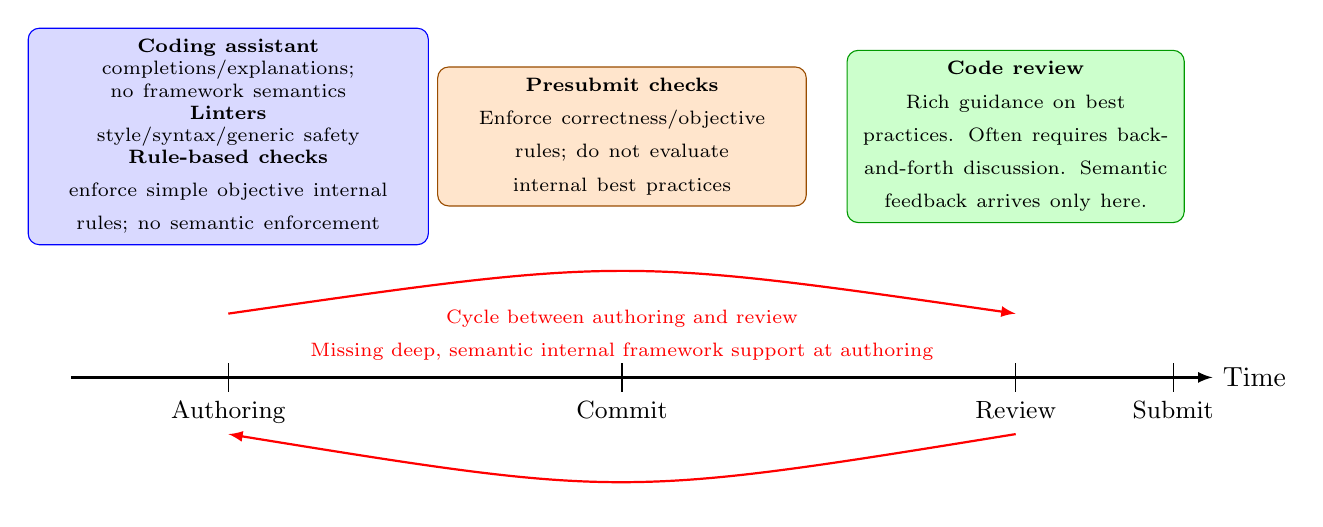
\begin{tikzpicture}[x=1.0cm,y=0.9cm,>=latex]
% Timeline axis
\draw[->,thick] (0,0) -- (14.5,0) node[right]{Time};
% Phase markers
\foreach \x/\name in {2/Authoring,7/Commit,12/Review,14/Submit} {
  \draw (\x,0.2) -- (\x,-0.2);
  \node[below] at (\x,-0.2) {\small \name};
}

% Feedback nodes (title + why not enough)
% Authoring: combined rectangle with two points
\node[draw=blue, fill=blue!15, rounded corners, align=center, inner sep=4pt, text width=4.8cm] at (2,3.4)
  {\scriptsize \textbf{Coding assistant}\\\scriptsize completions/explanations; no framework semantics\\ \textbf{Linters}\\\scriptsize style/syntax/generic safety\\\textbf{Rule-based checks}\\\scriptsize enforce simple objective internal rules; no semantic enforcement};

\node[draw=orange!60!black, fill=orange!20, rounded corners, align=center, inner sep=4pt, text width=4.4cm] at (7,3.4)
  {\scriptsize \textbf{Presubmit checks}\\\scriptsize Enforce correctness/objective rules; do not evaluate internal best practices};

\node[draw=green!60!black, fill=green!20, rounded corners, align=center, inner sep=4pt, text width=4.0cm] at (12,3.4)
  {\scriptsize \textbf{Code review}\\\scriptsize Rich guidance on best practices. Often requires back-and-forth discussion. Semantic feedback arrives only here. };

% no rectangle at Submit stage (no feedback)
% Loop arrows between Authoring and Review
% Cycle arrows (top above timeline, bottom below timeline)
\draw[->,red,thick] (2,0.9) .. controls (7,1.7) .. (12,0.9);   % top arc (Authoring -> Review)
\draw[->,red,thick] (12,-0.8) .. controls (7,-1.7) .. (2,-0.8); % bottom arc (Review -> Authoring)
\node[red,align=center] at (7,0.60) {\scriptsize Cycle between authoring and review\\\scriptsize Missing deep, semantic internal framework support at authoring};
\end{tikzpicture}
\caption{Current feedback across the development timeline.}
\label{fig:developer_workflow_feedback_timeline}
\end{figure}


\noindent As the timeline suggests, authoring tools provide helpful but limited coverage: \textbf{coding assistants and linters} improve style, syntax, and generic safety, and \textbf{rule‑based checks} can enforce simple, objective internal conventions (e.g., naming, imports). However, \textbf{none of these provide semantic enforcement of internal framework best practices at the point of writing}. At commit time, \textbf{presubmit checks} primarily ensure correctness rather than best‑practice conformance. The first truly \textbf{semantic, framework‑aware feedback} typically appears in \textbf{code review}, where it is rich but time‑bounded and variable—often prompting back‑and‑forth and rework.

\subsubsection{Impact of Delayed Feedback}

The current workflow introduces several challenges:

\begin{itemize}
\item \textbf{Inconsistent Quality Standards:} Lack of real-time guidance leads to variable adherence across teams.
\item \textbf{Prolonged Review Cycles:} Multiple iterations are required to fix issues discovered late.
\item \textbf{Technical Debt Accumulation:} Delayed feedback leads to inconsistencies and long-term maintenance costs.
\item \textbf{Developer Frustration:} Repetitive corrections decrease productivity.
\item \textbf{Increased Costs:} Late discovery of issues exponentially increases remediation effort.
\end{itemize}

\subsubsection{Opportunity for Framework-Specific AI Solutions}

The analysis reveals a clear opportunity for integrating framework-specific AI solutions. Combining the intelligence of market tools with the specificity required for internal frameworks, these solutions can deliver real-time, context-aware guidance directly in the coding phase.

Such a solution addresses the observed gap:

\begin{itemize}
\item Real-time adherence to internal framework best practices.
\item Integration directly into the developer workflow.
\item Proactive feedback that reduces review effort and technical debt.
\end{itemize}

This motivates the development of an LLM-powered assistant integrated into the coding phase within the \textbf{Integrated Development Environment (IDE)}. The IDE concentrates the artifacts and signals of software work (source files, diagnostics, version state, and developer intent), so in‑editor guidance shortens the loop between authoring and feedback and keeps advice anchored in local context.
\section{Project Requirements}

We now translate the identified opportunity into concrete requirements. The proposed solution integrates LLM-powered assistance directly into the developer workflow within the IDE to provide real-time, actionable guidance while maintaining performance, usability, and scalability.

\subsection{Use Case Analysis}

Understanding how developers will interact with the system is critical for designing effective functionality. Use case analysis provides a structured approach to capture user-system interactions, identify key actors, and define the boundaries of the system. This ensures that the system delivers targeted support precisely where it is needed during the active coding phase.

\begin{figure}[H]
    \centering
    \includegraphics[scale=0.6]{images/use_case_diagram.png}
    \caption{System Use Case Diagram}
    \label{fig:use_case_diagram}
    \end{figure}

Figure~\ref{fig:use_case_diagram} illustrates the core functionality of the system from the perspective of YouTube developers. The primary actor is the \textbf{YouTube Developer}, who interacts with the system through three main use cases:

\begin{enumerate}
\item \textbf{Request Code Analysis:} Trigger real-time evaluation of code for adherence to framework best practices.
\item \textbf{Review Violations and Explanations:} Inspect flagged violations, with clear, context-specific explanations provided by the system.
\item \textbf{Apply Suggested Fixes (Optional):} Accept, modify, or reject actionable AI-generated suggestions to improve code quality.
\end{enumerate}

This design ensures that developers remain in control of their workflow while benefiting from comprehensive, intelligent feedback. Optional scenarios, such as applying fixes, allow flexibility and respect developer autonomy. The use case diagram focuses on core interactions, leaving authentication and configuration workflows out of scope.

\subsection{Functional Requirements}

Based on the use cases and the gaps identified in existing tools, the system must provide the following core functionalities:

\begin{itemize}
\item \textbf{Detect Framework Violations:} Identify violations of internal YouTube framework best practices in real-time.
\item \textbf{Provide Contextual Explanations:} Deliver developer-friendly explanations that clarify why a particular pattern is problematic.
\item \textbf{Generate Actionable Fixes:} Suggest concrete AI-driven solutions aligned with framework conventions.
\item \textbf{Enable Developer Interaction:} Allow developers to accept, reject, or modify suggested fixes, maintaining workflow control.
\item \textbf{Maintain Contextual Relevance:} Ensure feedback remains accurate and properly anchored as code evolves.
\item \textbf{Seamless IDE Integration:} Embed within the existing internal IDE without disrupting normal development processes.
\end{itemize}

\subsection{Non-Functional Requirements}

In addition to core functionality, the system must satisfy broader quality criteria:

\begin{itemize}
\item \textbf{Performance:} Provide near real-time feedback to avoid interrupting workflow.
\item \textbf{Scalability:} Efficiently handle large codebases and multiple simultaneous users.
\item \textbf{Maintainability:} Make it easy to modify, refactor, and repair existing components (rules, prompts, pipelines) with clear abstractions, tests, and documentation.
\item \textbf{Reliability:} Operate robustly in production with minimal downtime.
\item \textbf{Security and Privacy:} Comply with organizational policies, safeguarding code and data.
\item \textbf{Usability:} Deliver concise, context-aware, and minimally intrusive feedback.
\item \textbf{Extensibility:} Allow adding new capabilities (rules, models, tools, IDE touchpoints) via well-defined extension points without changing existing components.
\end{itemize}

Table~\ref{tab:extended_requirements} summarizes functional and non-functional requirements.

\begin{table}[H]
\centering
\caption{Summary of Project Requirements}
\label{tab:extended_requirements}
\begin{tabular}{|p{3cm}|p{11cm}|}
\hline
\textbf{Requirement Type} & \textbf{Description} \\
\hline
Functional & Detection, explanations, fixes, interaction, context, IDE integration \\
\hline
Non-Functional & Performance, scalability, maintainability, reliability, security, usability, extensibility \\
\hline
\end{tabular}
\end{table}


These requirements directly address the gaps identified in both market and environment-specific solutions. By embedding proactive, context-aware feedback into the coding workflow, the system:

\begin{itemize}
\item Reduces framework-specific errors during development.
\item Improves adherence to YouTube internal standards.
\item Enhances developer productivity by providing guidance in real-time.
\end{itemize}

\section*{Conclusion}

This chapter set the foundations: AI, LLMs, and agents; why agents are needed; and why the IDE is the right place for real‑time guidance. It mapped AI’s role across the SDLC, reviewed market and environment approaches, and showed a gap in enforcing internal framework best practices at authoring. From this analysis, it defined the opportunity and the project’s requirements. The next chapter presents the system design and architecture that realizes authoring‑time, framework‑aware guidance in the IDE.






%==============================================================================
\end{spacing}


